%!TEX root = ../thesis.tex
%******************************************************************************
\chapter{Background}\label{ch:background}
%******************************************************************************

\section{Batch processing}\label{sec:batch_processing}
The traditional operation paradigm of a system for bulk data processing is batch processing (see Figure \ref{fig:batch_processing}). A batch processing system is an application that processes bulk data without user interaction. Input and output data is usually organised in records using a file- or database-based interface. In the case of a file-based interface, the application reads a record from the input file, processes it and writes the record to the output file.
\begin{figure}[h!]
	\centering
	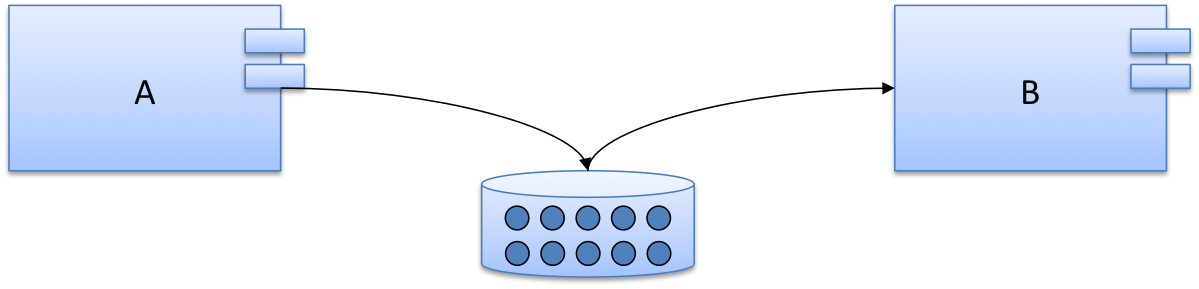
\includegraphics[width=\columnwidth]{batch}
	\caption{Batch processing}
	\label{fig:batch_processing}
\end{figure}

A batch processing system exhibits the following key characteristics:
\begin{itemize}
	\item \textbf{Bulk processing of data}\\
	A Batch processing system processes several gigabytes of data in a single run thus providing a high throughput. Multiple systems are running in parallel controlled by a job scheduler to speed up processing. The data is usually partitioned and sorted by certain criteria for optimized processing. For example, if a batch only contains data for a specific product, the system can pre-load all necessary reference data from the database to speed up the processing.
	\item \textbf{No user interaction}\\
	There is no user interaction needed for the processing of data. It is impossible due to the amount of data being processed.
	\item \textbf{File- or database-based interfaces}\\
	Input data is read from the file system or a database. Output data is also written to files on the file system or a database. Files are transferred to the consuming systems through FTP by specific jobs.
	\item \textbf{Operation within a limited timeframe}\\
	A batch processing system often has to deliver its results in a limited timeframe due to \ac{SLA} with consuming systems.
	\item \textbf{Offline handling of errors}\\
	Erroneous records are stored to a specific persistent memory (file or database) during operation and are processed afterwards.
\end{itemize}
Applications that are usually implemented as batch processing systems are billing systems for telecommunication companies used for mediating, rating and billing of call events.

\section{Message-base processing}\label{sec:message_processing}
Messaging facilitates the integration of heterogeneous applications using asynchronous communication. Applications are communicating with each other by sending messages (see Figure \ref{fig:message_based_processing}). A messaging server or message-oriented middleware handles the asynchronous exchange of messages including an appropriate transaction control \cite{conrad2006enterprise}.

\begin{figure}[h!]
	\centering
	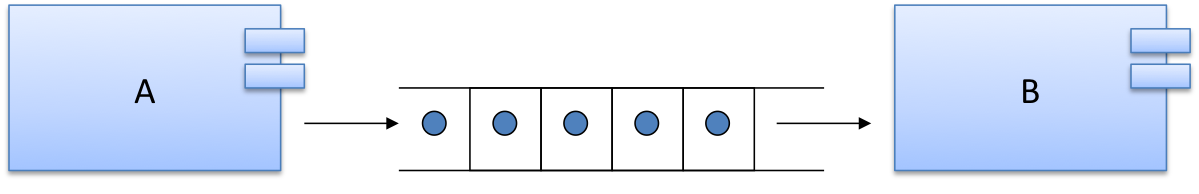
\includegraphics[width=\columnwidth]{esb}
	\caption{Message-based processing}
	\label{fig:message_based_processing}
\end{figure}

Hohpe et al.\cite{Hohpe:2003fk} describe the following basic messaging concepts:
\begin{itemize}
	\item \textbf{Channels}\\
	Messages are transmitted through a channel. A channel connects a message sender to a message receiver.
	\item \textbf{Messages}\\
	A message is packet of data that is transmitted through a channel. The message sender breaks the data into messages and sends them on a channel. The message receiver in turn reads the messages from the channel and extracts the data from them.
	\item \textbf{Pipes and Filters}\\
	A message may pass through several processing steps before it reaches its final destination. Multiple processing steps are chained together using a pipes and filters architecture.
	\item \textbf{Routing}\\
	A message may have to go through multiple channels before it reaches its destination. A message router acts as a filter and is capable of routing a message to the next channel or to another message router.
	\item \textbf{Transformation}\\
	A message can be transformed by a message translator if the message sender and receiver do not agree on the format for the same conceptual data.
	\item \textbf{Endpoints}\\
	A message endpoint is a software layer that connects arbitrary applications to the messaging system.
\end{itemize}

Message-based systems are able to provide near-time processing of data due to their lower latency compared with batch processing systems. The advantage of a lower latency comes with a performance cost in regard to a lower throughput because of the additional overhead for each processed message. Every message needs amongst others to be serialised and deserialised, mapped between different protocols and routed to the appropriate receiving system.

\section{Latency vs. Throughput}\label{sec:latency_throughput}
Throughput and latency are performance metrics of a system. The following definitions of throughput and latency are used in this paper:
\begin{itemize}
	\item \textbf{Maximum Throughput}\\
	The number of events the system is able to process in a fixed timeframe.
 	\item \textbf{Ent-to-end Latency}\\
	The period of time between the occurrence of an event and its processing. End-to-end latency refers to the total latency of a complete business process implemented by multiple subsystems. The remainder of this paper focusses on end-to-end latency using the general term latency as an abbreviation.
\end{itemize}
\subsection{Batch processing}
A business process, such as billing, implemented by a system using batch processing exhibits a high end-to-end latency. For example, consider the following billing system:
\begin{itemize}
	\item Customers are billed once per month
	\item Customers are partitioned in 30 billing groups
	\item The billing system processes 1 billing group per day, running 24h under full load.
\end{itemize}

In this case, the mean time for a call event to be billed by the billing system is $1/2$ month. That is, the mean end-to-end latency of this system is $1/2$ month.

\begin{figure}[h!]
	\centering
	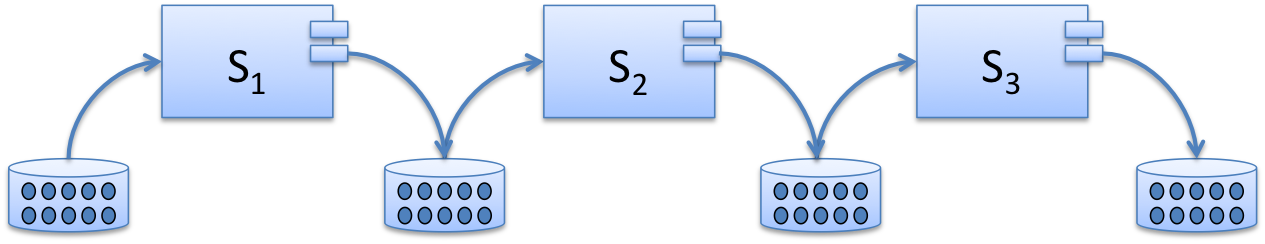
\includegraphics[width=\columnwidth]{latency_throughput1}
	\caption{Batch processing system comprised of three subsystems}
	\label{fig:batch_processing_latency}
\end{figure}

Assuming the system $S_{Batch}$ which is comprised of $N$ subsystems $S_1$, $S_2$, \ldots, $S_N$ (see Figure \ref{fig:batch_processing_latency} for an example with $N=3$):
\begin{displaymath}
S_{Batch} = \{S_1, S_2, \ldots, S_N\}
\end{displaymath}
The subsystem $S_i$ reads its input data from the database $DB_i$ in one chunk, processes it and writes the output to the database $DB_{i+1}$. When $S_i$ has finished the processing, the next subsystem $S_{i+1}$ reads the input data from $DB_{i+1}$, processes it and writes the output to $DB_{i+2}$, which in turn is read and processed from subsystem $S_{i+3}$ and so on.

The latency $L_{E_{S_{Batch}}}$ of a single event processed by the system $S_{Batch}$ is determined by the total processing time $PT_{S_{Batch}}$, which is the sum of the processing time $PT_i$ of each subsystem $S_i$:
\begin{displaymath}
L_{E_{S_{Batch}}} = PT_{S_{Batch}} = \sum_{i=1}^N PT_i
\end{displaymath}
where $N$ is the number of subsystems.

The processing time $PT_i$ of the subsystem $S_i$ is the sum of the processing time of each event $PT_{E_{j}}$ and the additional processing overhead $OH_i$, which includes the time spent for reading and writing the data, opening and closing transactions, etc:
\begin{displaymath}
PT_i = \left(\sum_{j=1}^M PT_{E_{j}}\right) + OH_i
\end{displaymath}
where $M$ is the number of events.

To allow for near-time processing, it is necessary to decrease the latency $L_{E_S}$ of a single event. This is can be achieved by using message-based processing instead of batch processing.

\subsection{Message-based processing}
The subsystem $S_i$ of a message-based system $S_{Message}$ reads a single event from its input message queue $MQ_i$, processes it and writes it to the output message queue $MQ_{i+1}$. As soon as the event is written to the message queue $MQ_{i+1}$, it is read by the subsystem $S_{i+1}$, which processes the event and writes to the message queue $MQ{i+2}$ and so on (see Figure \ref{fig:message_based_latency}).

The latency $L_{E_{S_{Message}}}$ of a single event processed by the system $S_{Message}$ is determined by the total processing time $PT_{E_{S_{Message}}}$ of this event, which is the sum of the processing time $PT_{E_i}$ and the processing overhead $OH_{E_{i}}$ for the event of each subsystem:
\begin{displaymath}
L_{E_{S_{Message}}} = PT_{E_{S_{Message}}} = \sum_{i+1}^N (PT_{E_i} + OH_{E_i})	
\end{displaymath}
where $N$ is the number of subsystems. Please note that the wait time of the event is assumed to be 0 for simplification.

The processing overhead $OH_{E_i}$ includes amongst others the time spent for unmarshalling and marshalling, protocol mapping and opening and closing transactions, which is done for every processed event.

\begin{figure}[h!]
	\centering
	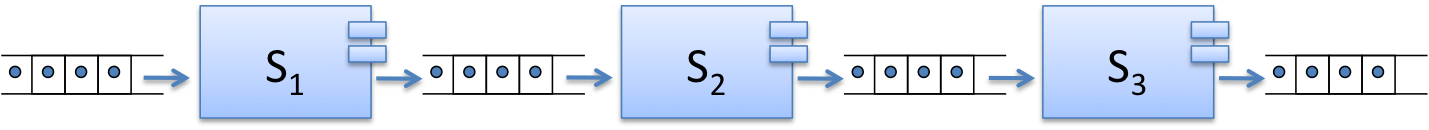
\includegraphics[width=\columnwidth]{latency_throughput2}
	\caption{Message-based system comprised of three subsystems}
	\label{fig:message_based_latency}
\end{figure}

Since the processing time $PT_{E_{S_{Message}}}$ of a single event is much shorter than the total processing time $PT_{S_{Batch}}$ of all events, the latency $L_{E_{S_{Message}}}$ of a single event using a message-based system is much smaller than the latency $L_{E_{S_{Batch}}}$ of a single event processed by a batch-processing system.
\begin{displaymath}
PT_{E_{S_{Message}}} < PT_{S_{Batch}} \Rightarrow L_{E_{S_{Message}}} < L_{E_{S_{Batch}}}
\end{displaymath}

Message-based processing adds an overhead to each processed event in contrast to batch processing, which adds a single overhead to each processing cycle. Hence, the accumulated total processing overhead $OH_{S_{Message}}$ of a message-based system $S_{Message}$ for processing $m$ events is larger than the total processing overhead of a batch processing system:
\begin{displaymath}
OH_{S_{Message}} = \sum_{i=1}^n OH_{E_i} * m > OH_{S_{Batch}} = \sum_{i=1}^n OH_i
\end{displaymath}
A message-based system, while having a lower end-to-end latency, is not able to process the same amount of events in the same time as a batch processing system and therefore cannot provide the same maximum throughput.

\begin{figure}[h!]
	\centering
	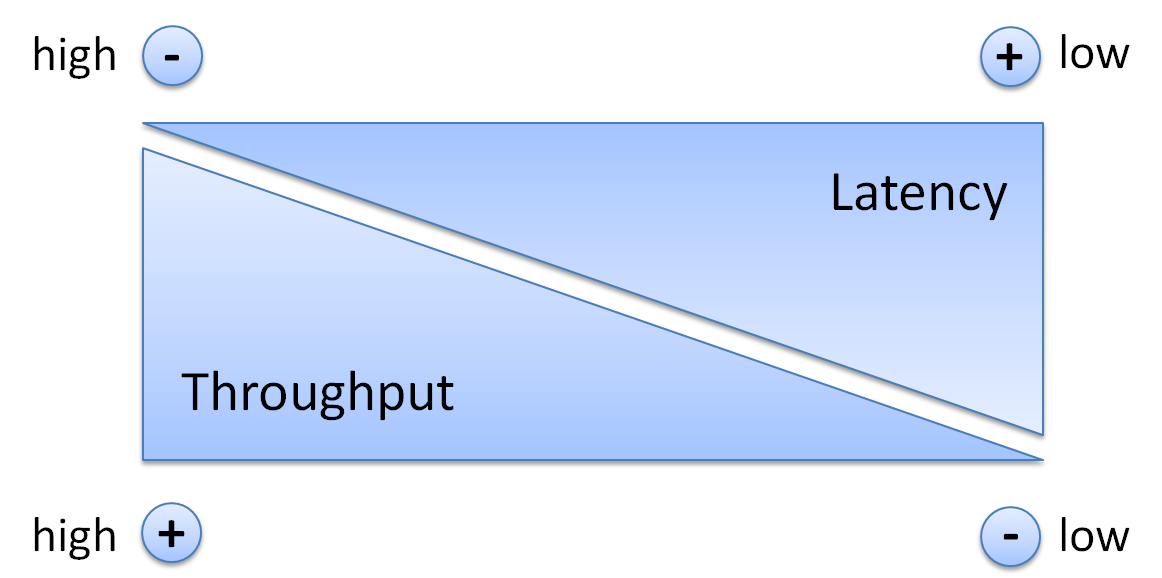
\includegraphics[width=\columnwidth]{latency_vs_throughput}
	\caption{Latency and throughput are opposed to each other}
	\label{fig:latency_vs_throughput}
\end{figure}

From this follows that latency and throughput are opposed to each other (see Figure \ref{fig:latency_vs_throughput}). High throughput, as provided by batch processing, leads to high latency, which impedes near-time processing. On the other hand, low latency, as provided by a message-based system, cannot provide the throughput needed for bulk data processing because of the additional overhead for each processed event.